% !TEX TS-program = xelatex
% !TEX encoding = UTF-8
% !Mode:: "TeX:UTF-8"

\documentclass[onecolumn, oneside, ctexart]{SUSTechHomework}
\setlength{\parindent}{2em}
\linespread{1.5}

\coursecode{CS305}
\coursename{Computer Networking}
\title{Program Assignment 1}
\date{Mar. 27, 2022}

\begin{document}
\maketitle
\toc

\section{Screenshots to Prove Workability}
\subsection{Correctness}
The following five test cases all runs as expected, the result is similar  to the reference answer and \textit{dig @114.114.115.115}. Please also notice the warning: \emph{recursion requested but not available}, which was what we want.\\~\\
\centerline{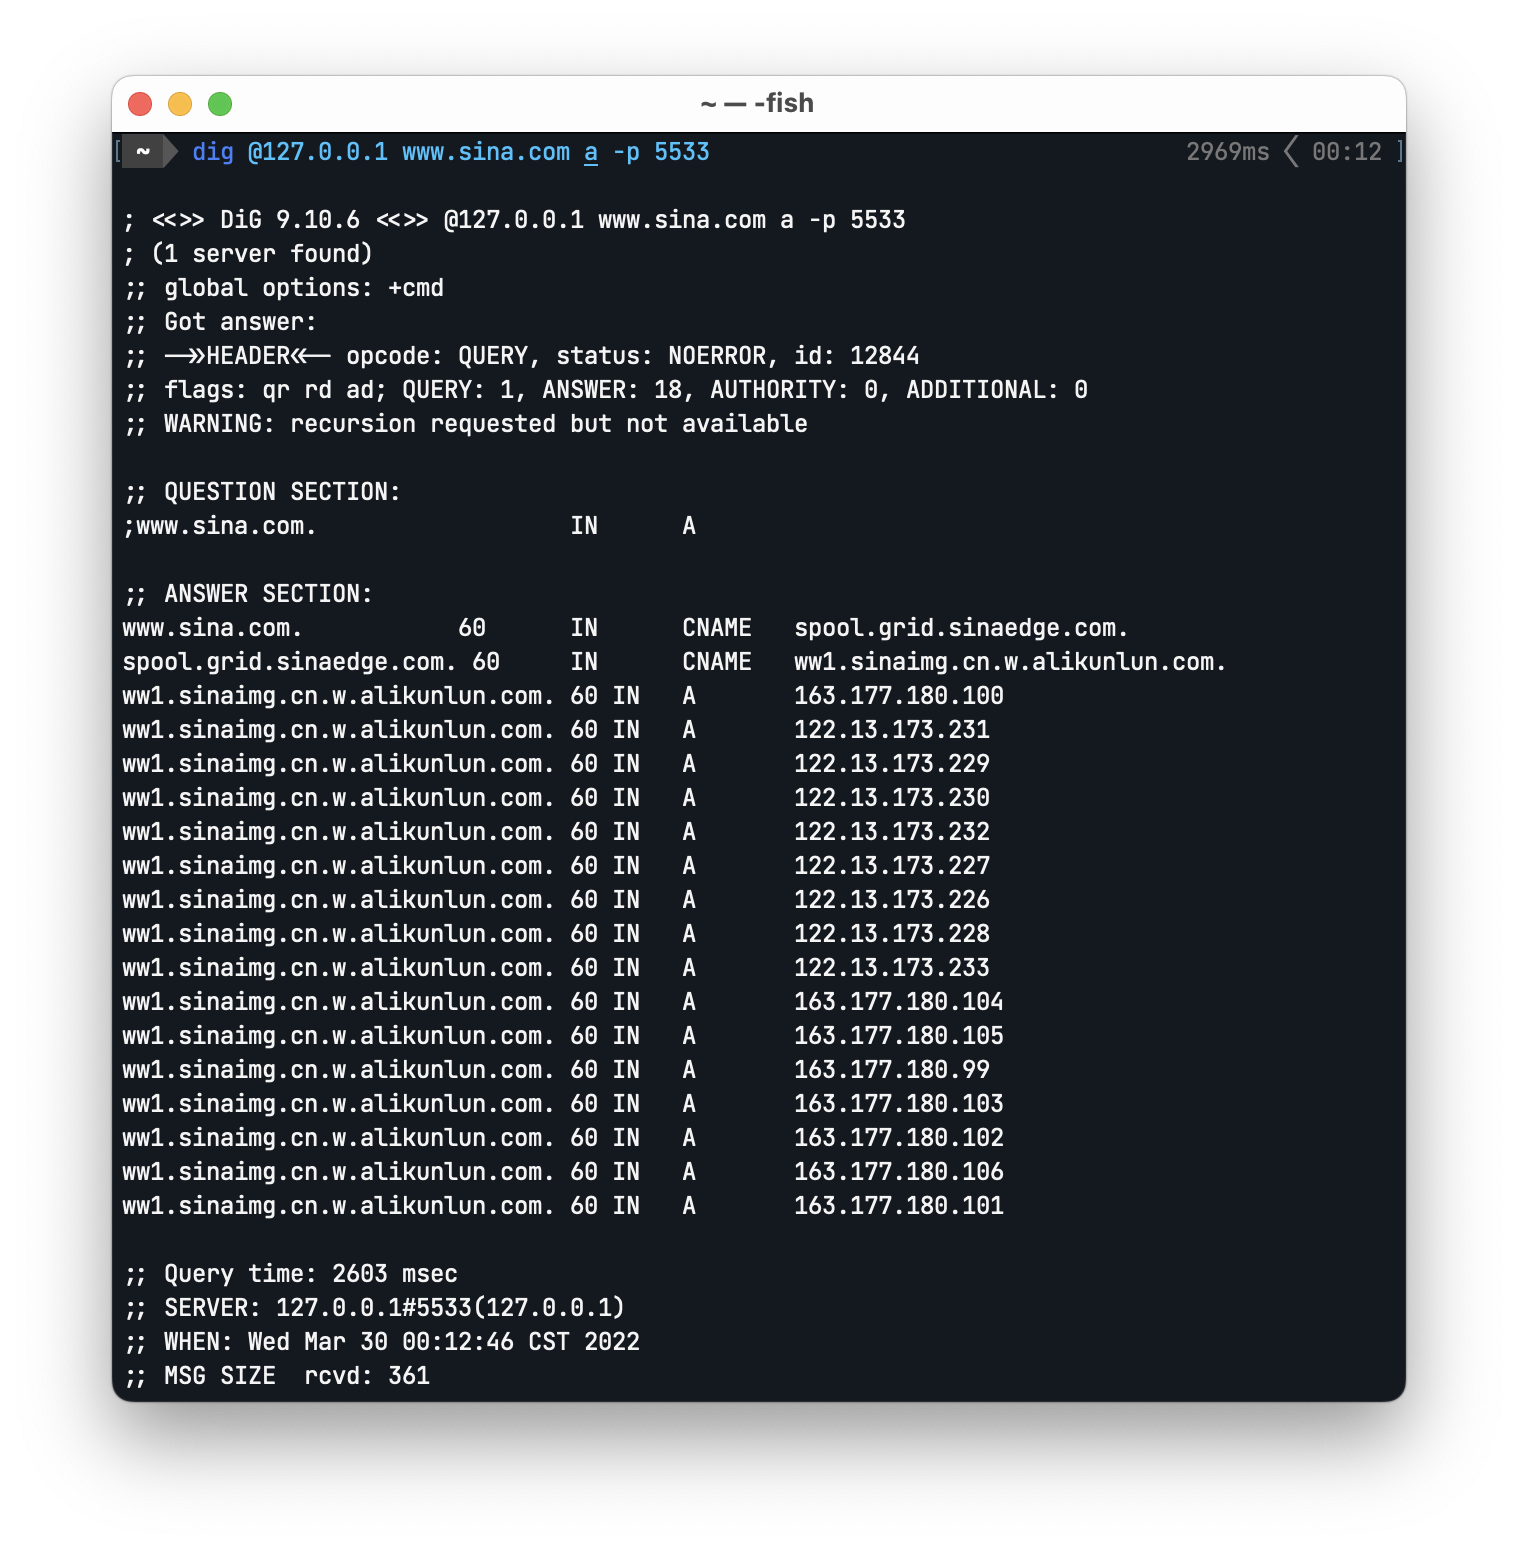
\includegraphics[height=6cm]{fig/c0}\quad
			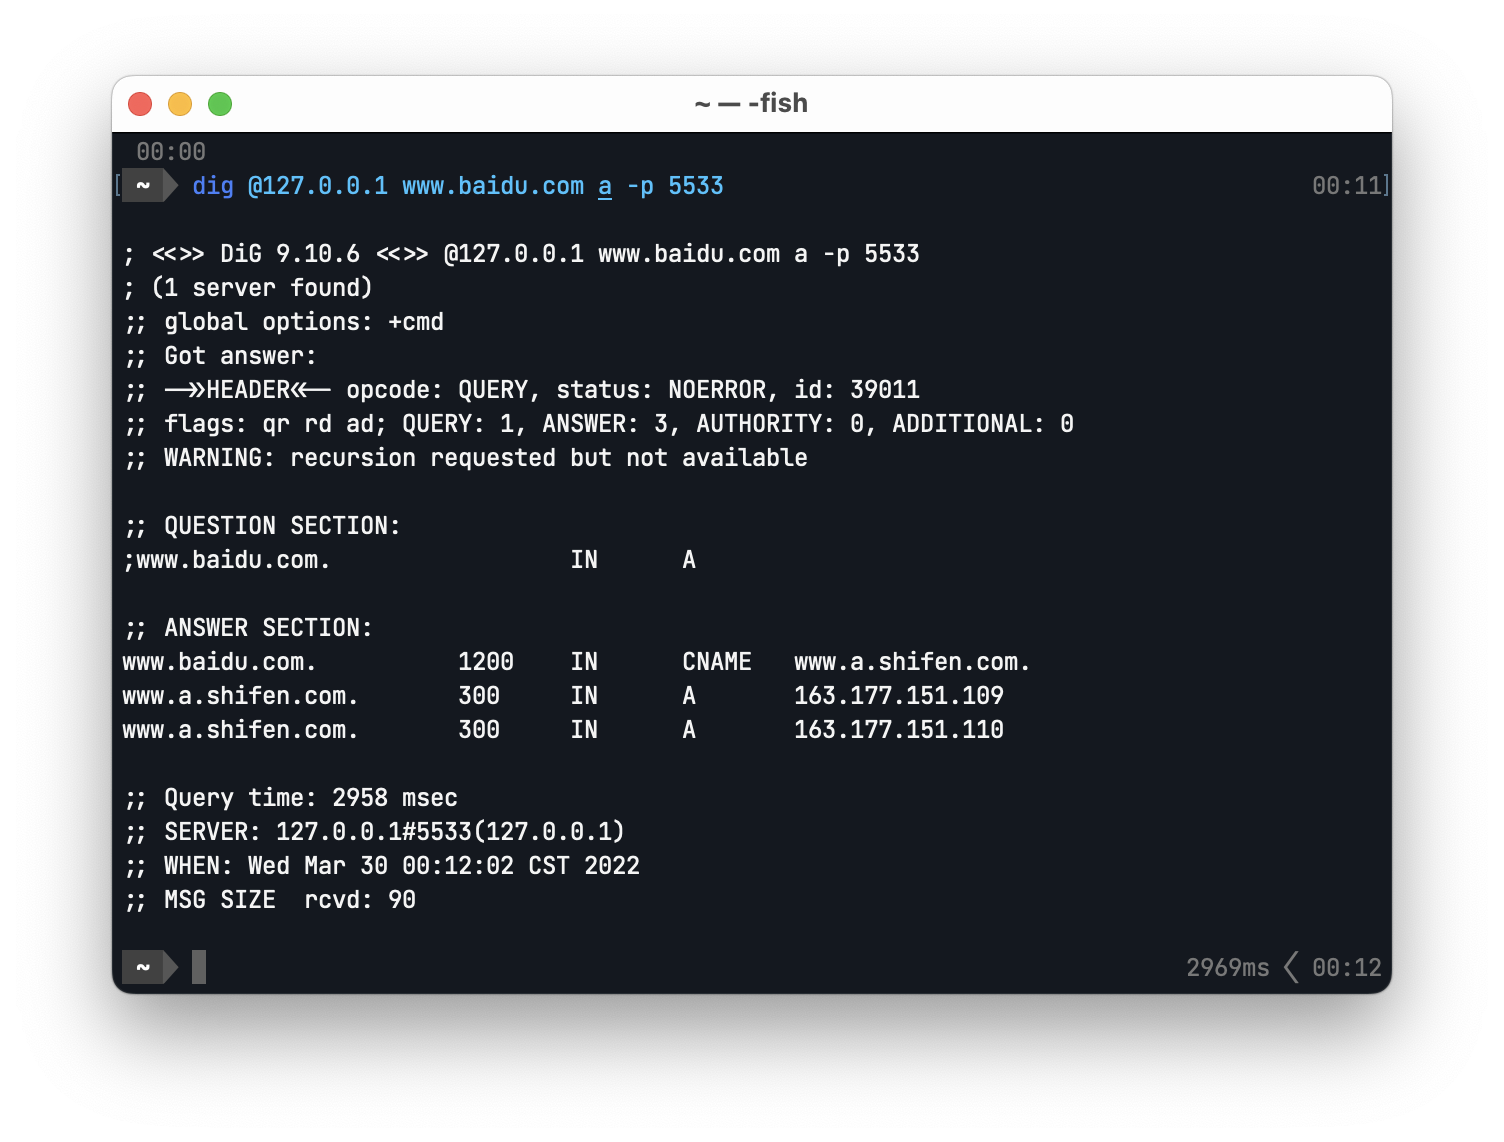
\includegraphics[height=6cm]{fig/c1}}\\
\centerline{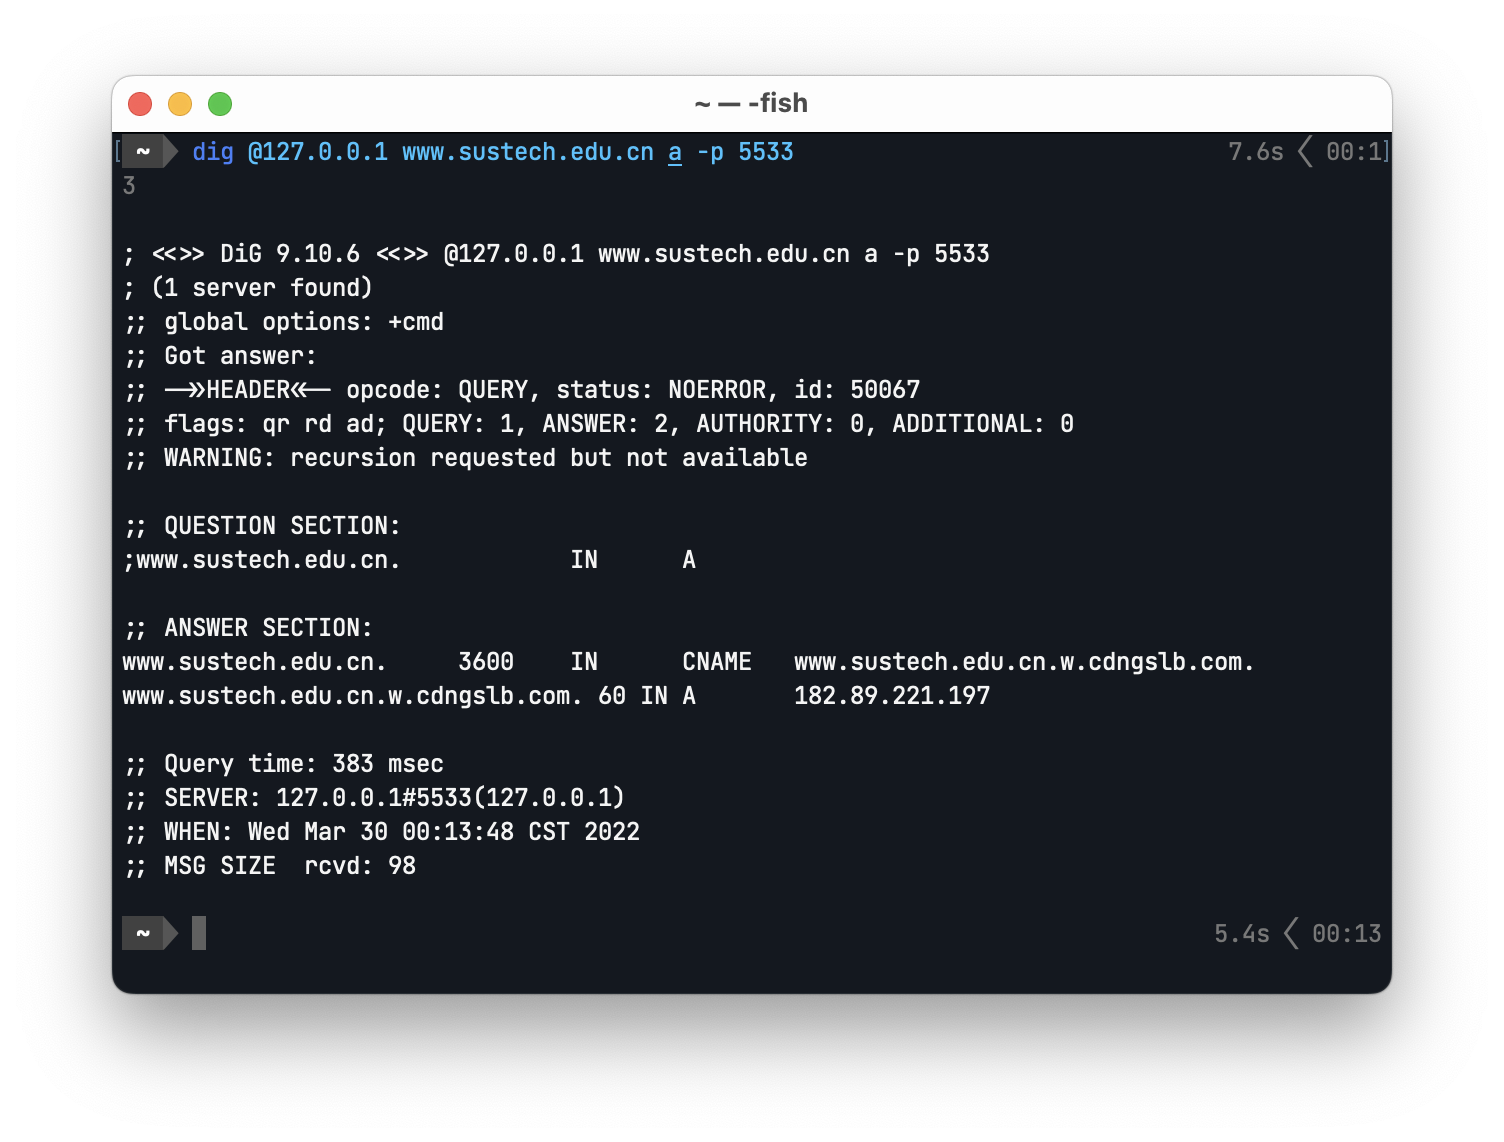
\includegraphics[height=6cm]{fig/c2}\quad
			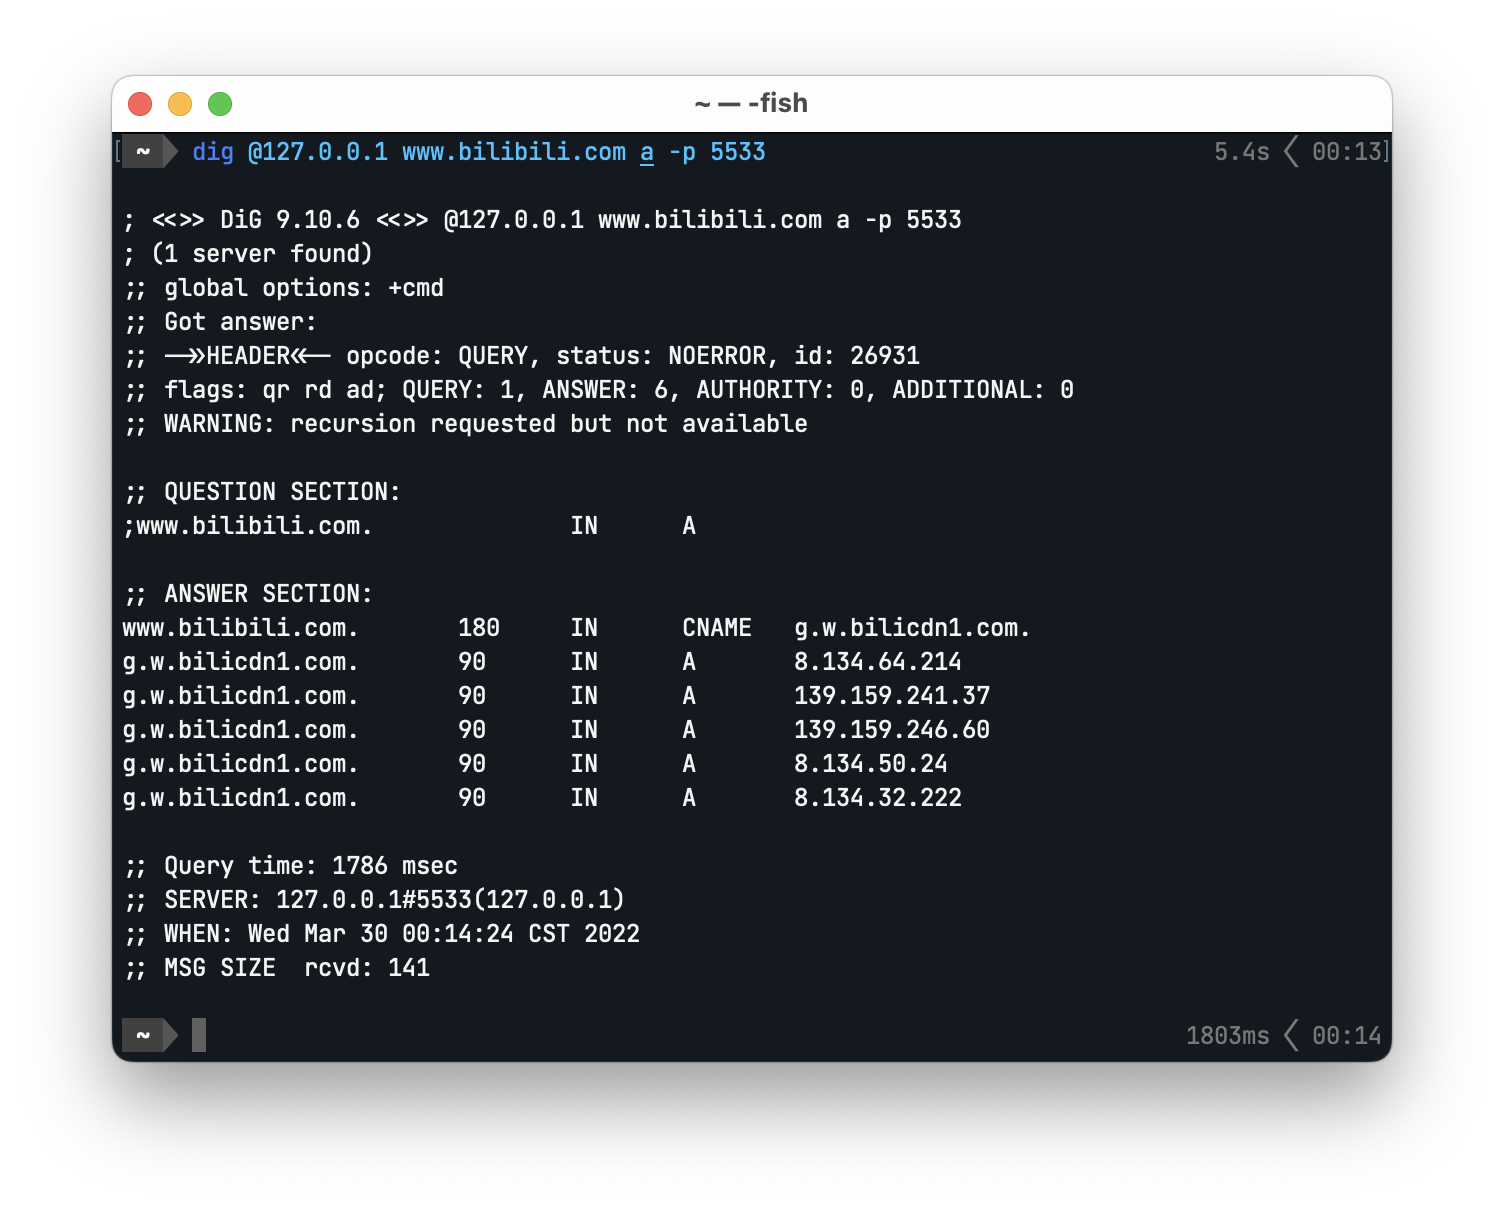
\includegraphics[height=6cm]{fig/c3}}\\
\centerline{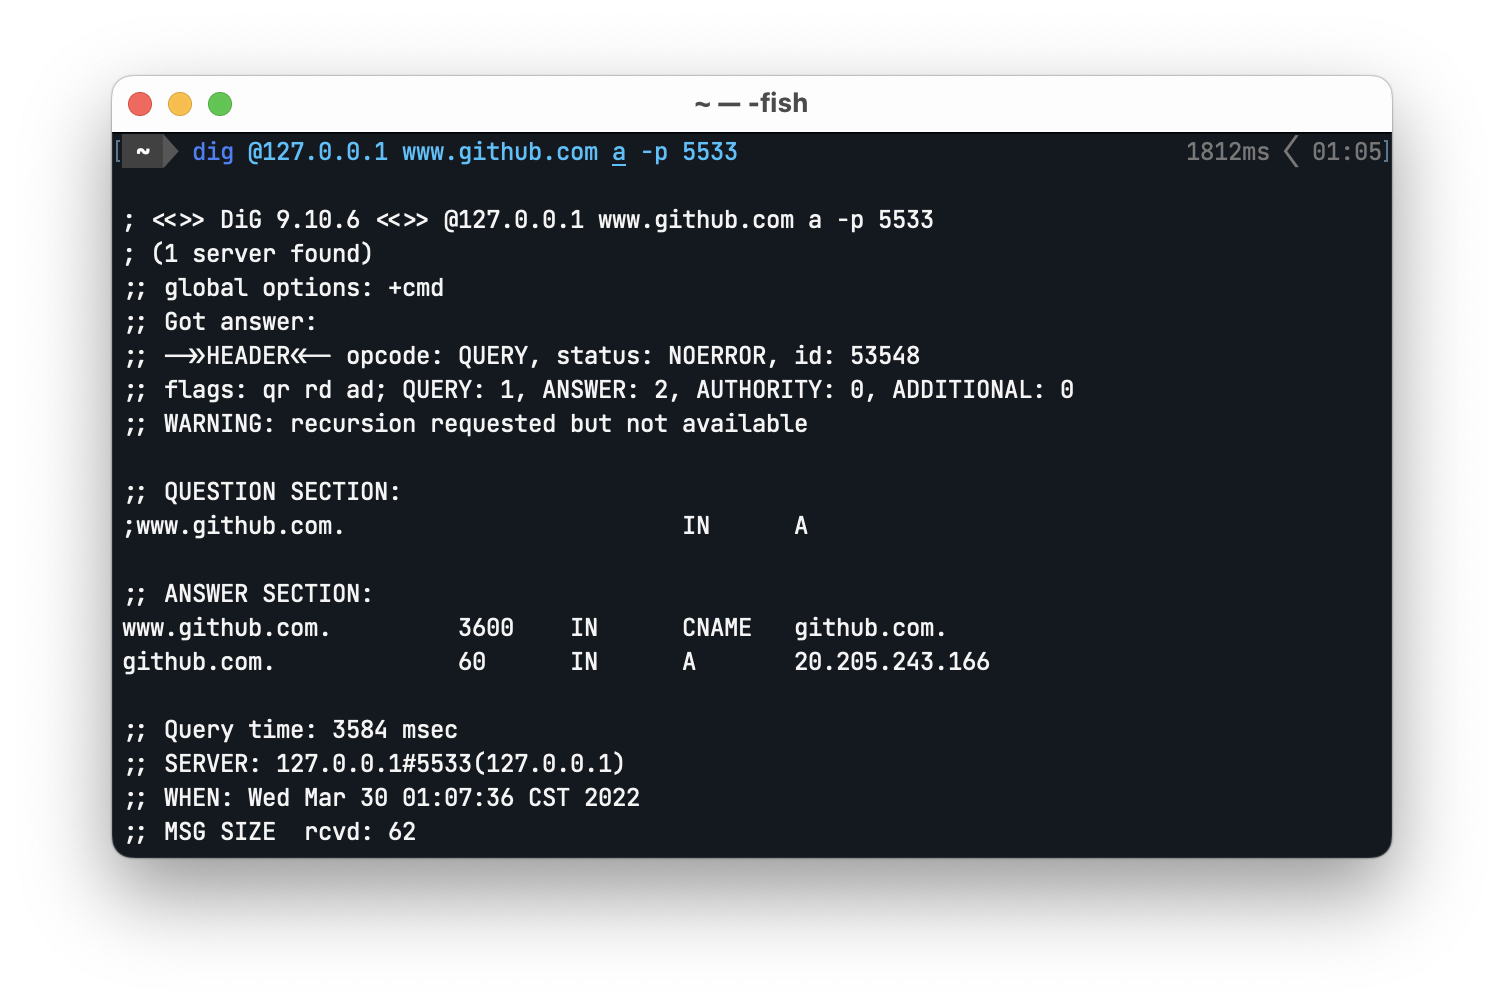
\includegraphics[height=6cm]{fig/c4}}

\subsection{Read from Cache}
Please see section \ref{reply a cache}. But note that, if a query does need a long time to finish, dig may close the connect due to timeout. But the next same query can fortunately hit the cache and get the result.

\subsection{Error Handling}
When the network condition is awful, DNS queries may often got timeout. The local DNS server will keep retrying several times (here is set as 10), if it still fails, return no answer, and set the status as 3: NXDOMAIN to indicate an error. As for wrong query names, it will not retry (unless a previous timeout before knowing the query name is not found) and return not found, with status NXDOMAIN.\\~\\
\centerline{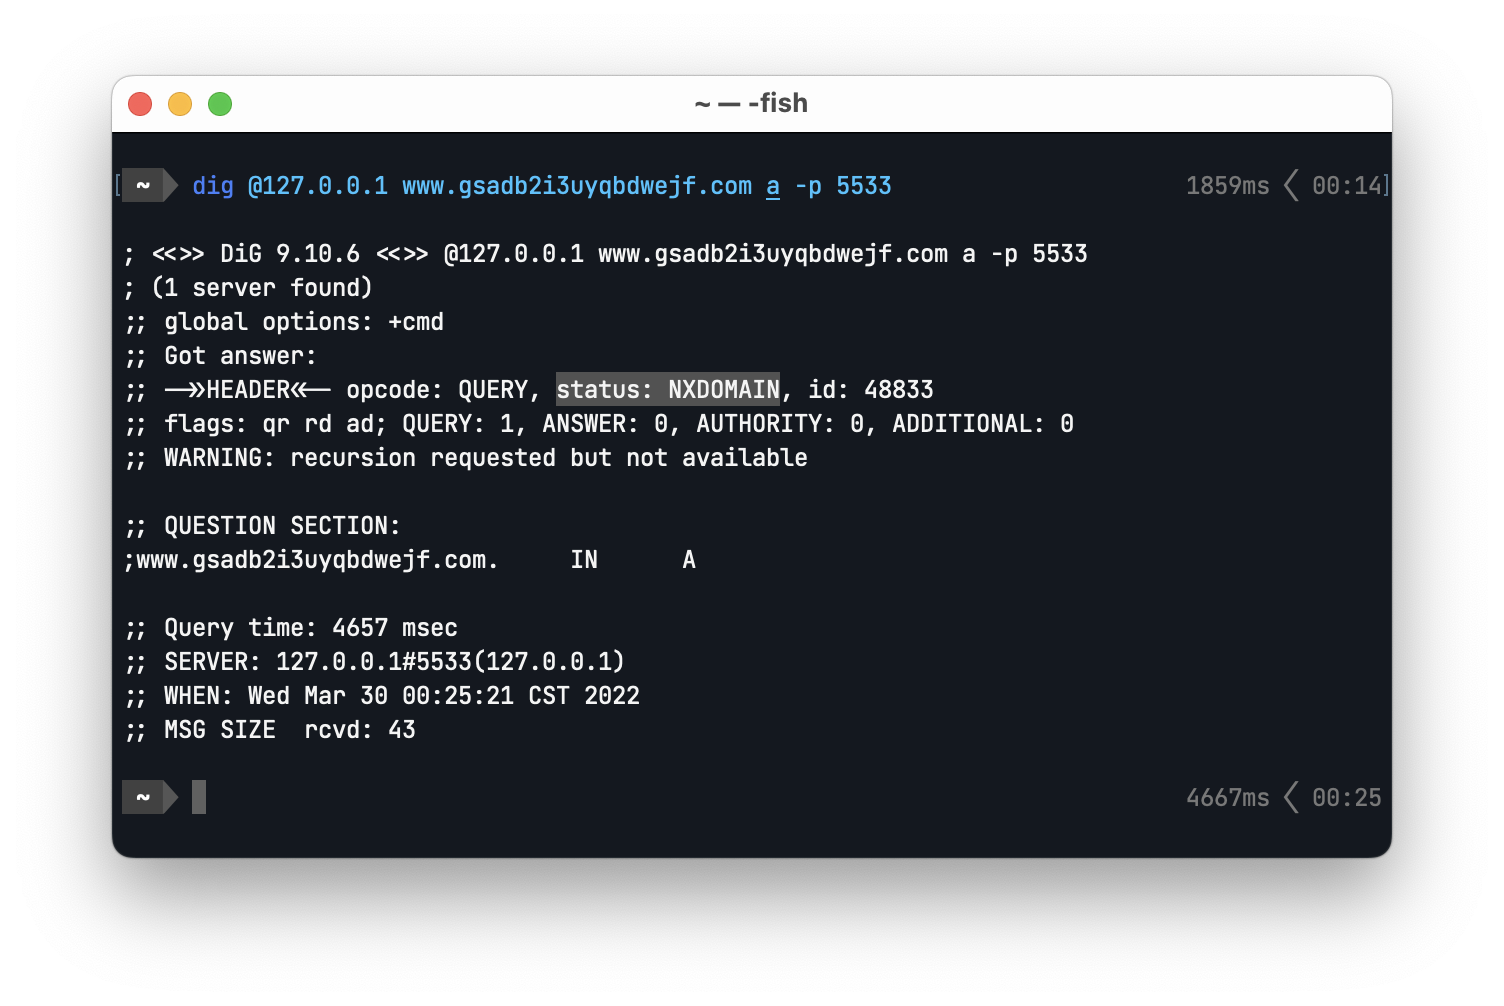
\includegraphics[height=5.2cm]{fig/e1}\quad
			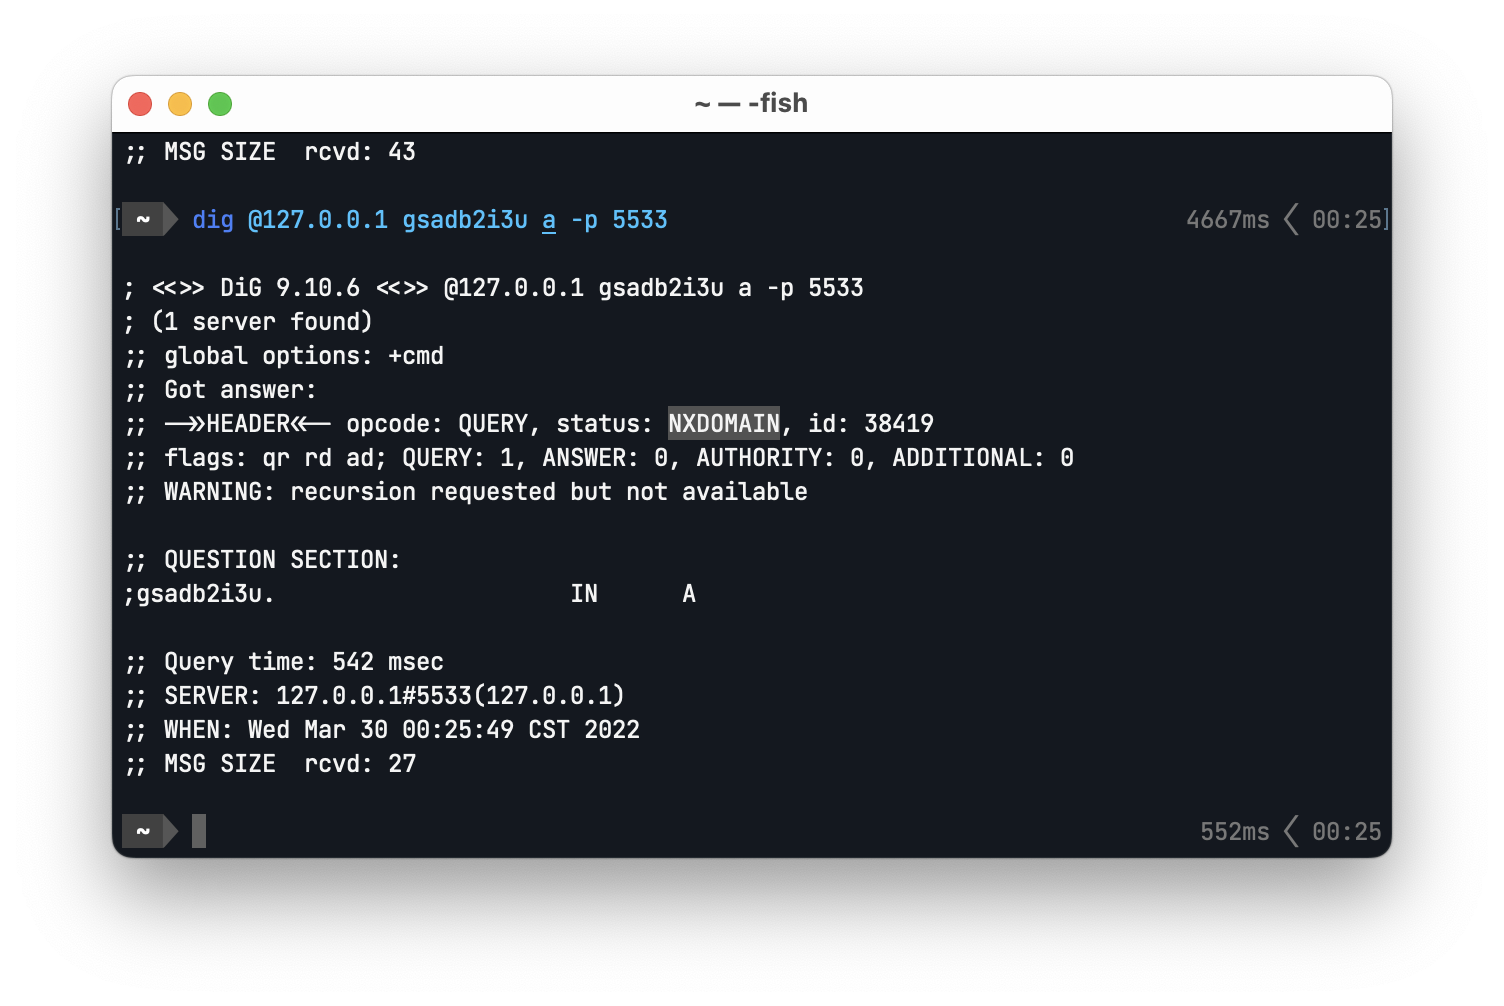
\includegraphics[height=5.2cm]{fig/e2}}

\subsection{Iterative Query}
The following Wireshark screenshots analyzes the process of an iterative query. The DNS server (172.20.10.3) first ask the root server (192.33.4.12) about the IP address of www.github.com, but it doesn't know, and provides TLD servers' NS records in authoritative nameservers' section, indicate our DNS server to take the same query name to the TLD servers. Note that in the additional section, the root server also provides their A records, we can therefore skip a query for TLD servers and straightly go for them.\\~\\
\centerline{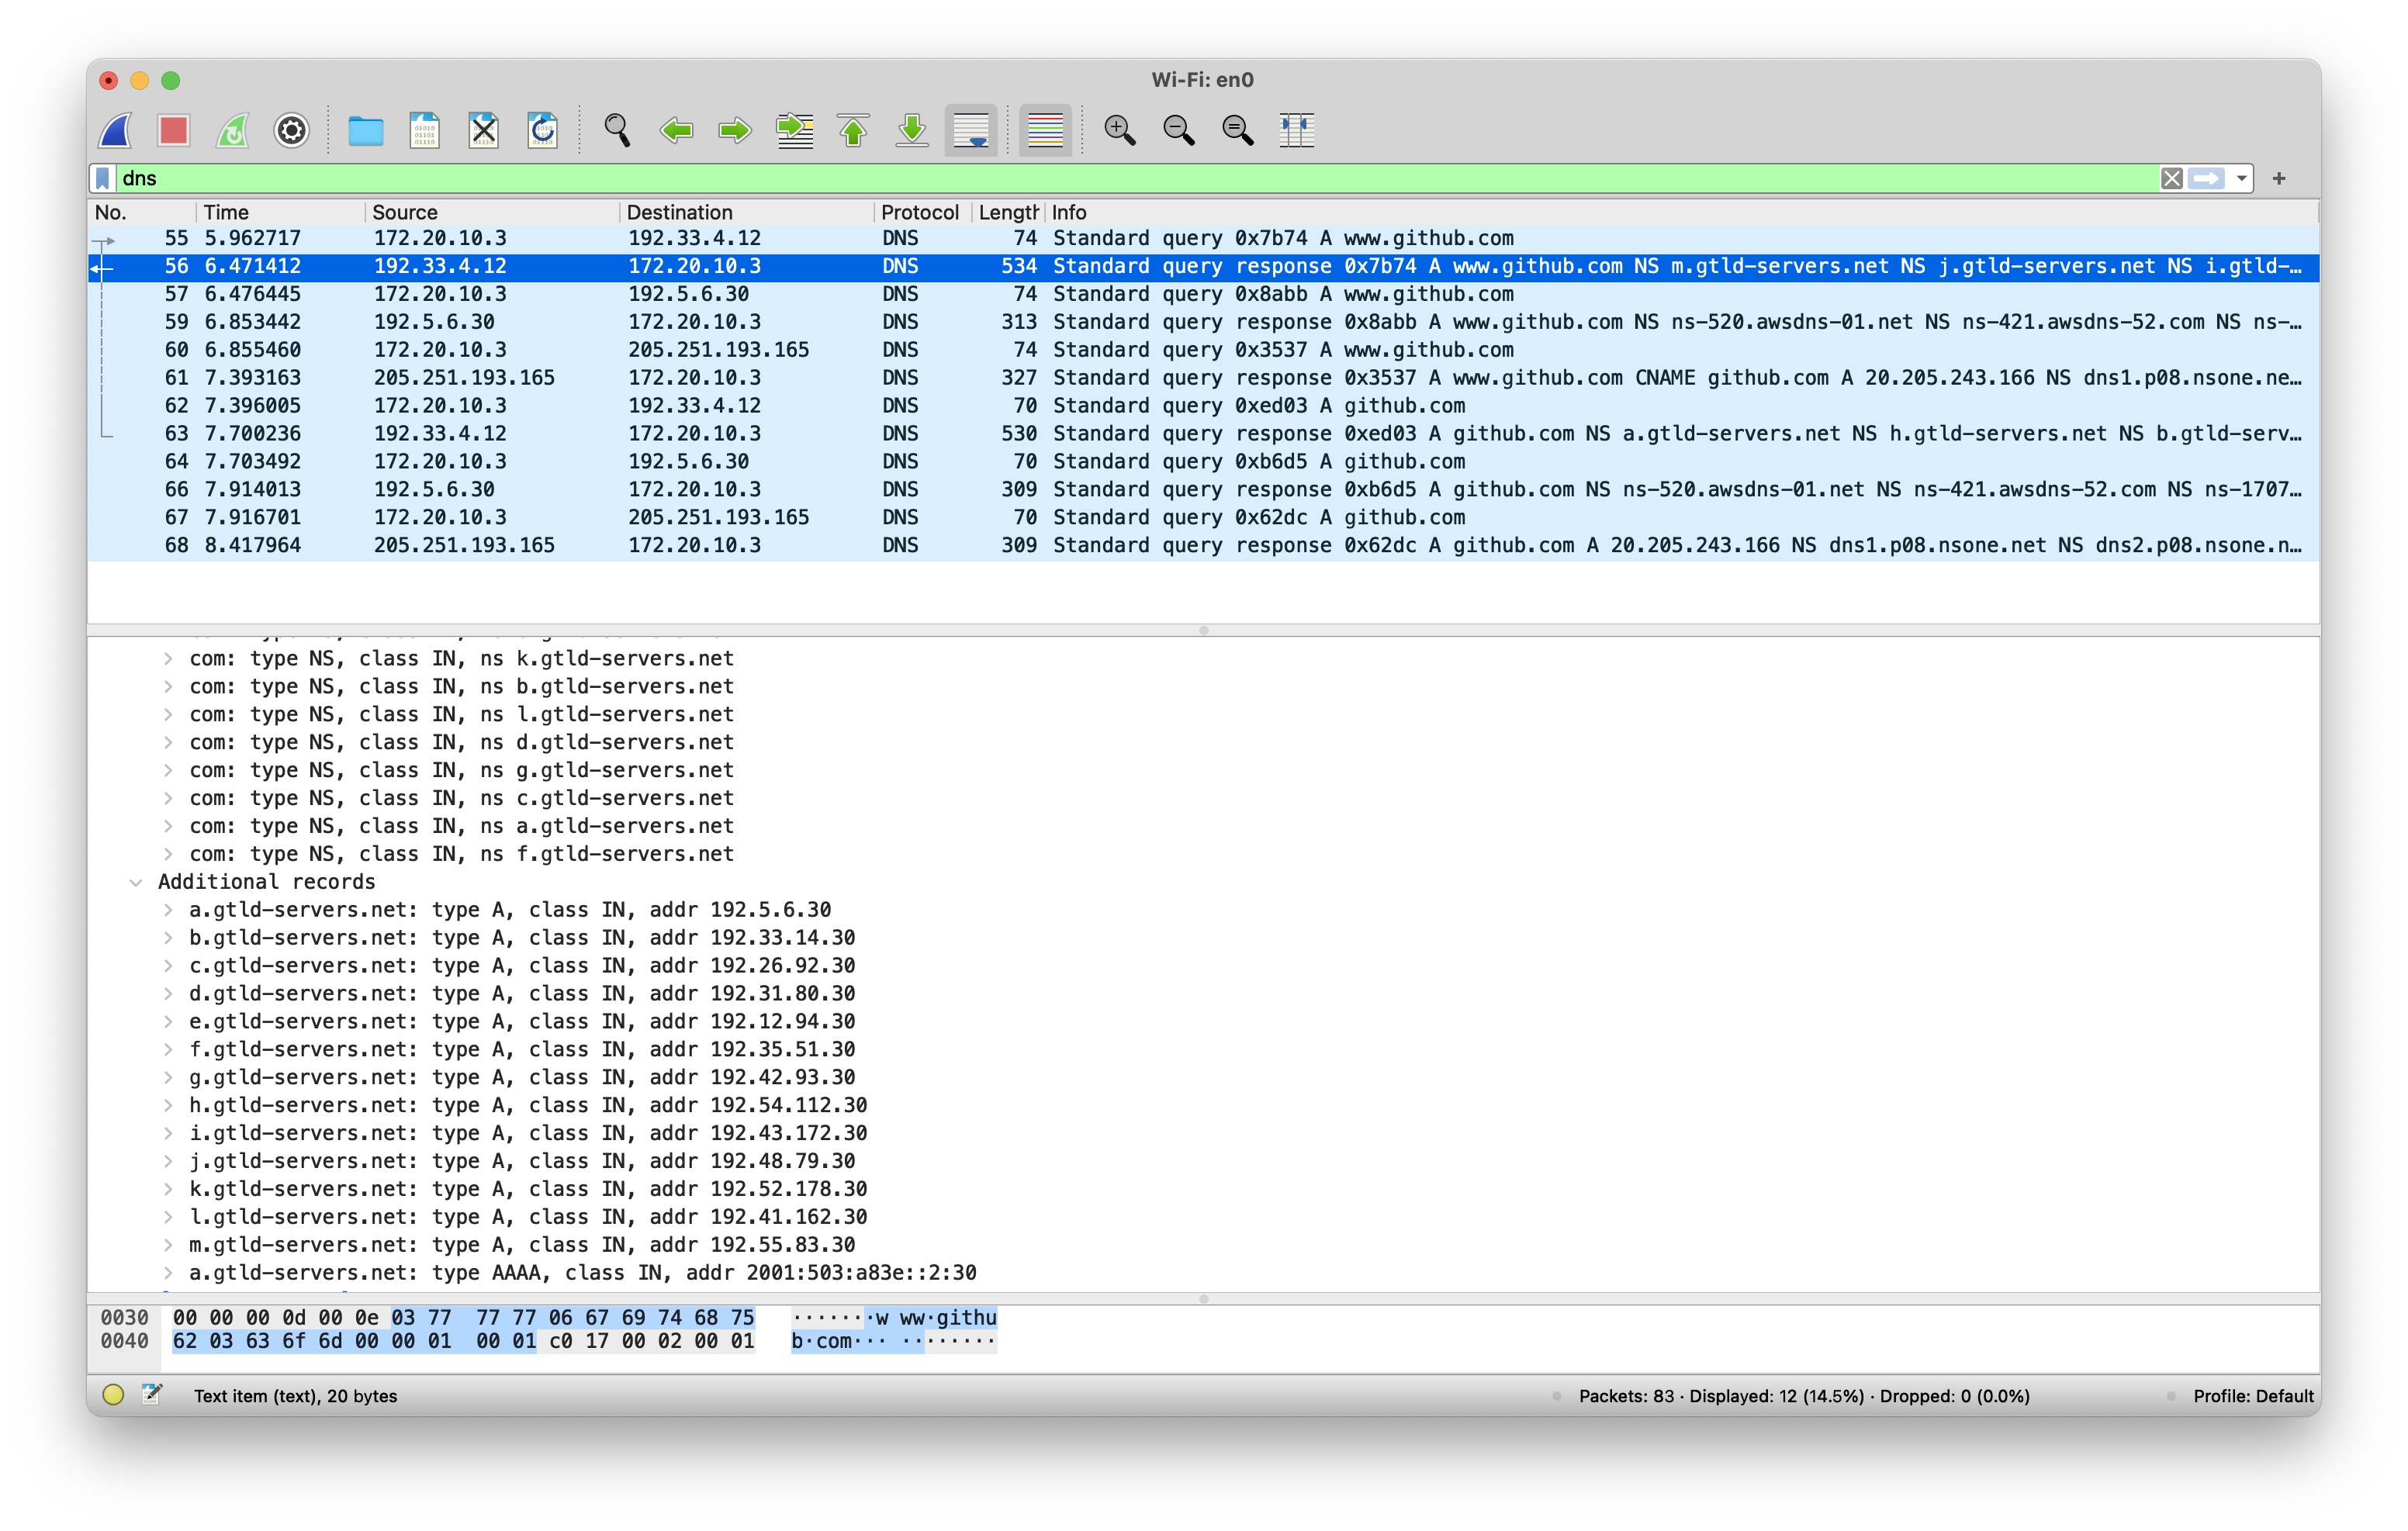
\includegraphics[height=6.2cm]{fig/w1}}
\par Our server happily take www.github.com to ask TLD 192.5.6.30, it also have no idea about the IP address, but it redirected our server to the authoritative server of GitHub, ns-520.awsdns-01.net etc., and provided an A record for one authoritative server, let's go for it.\\~\\
\centerline{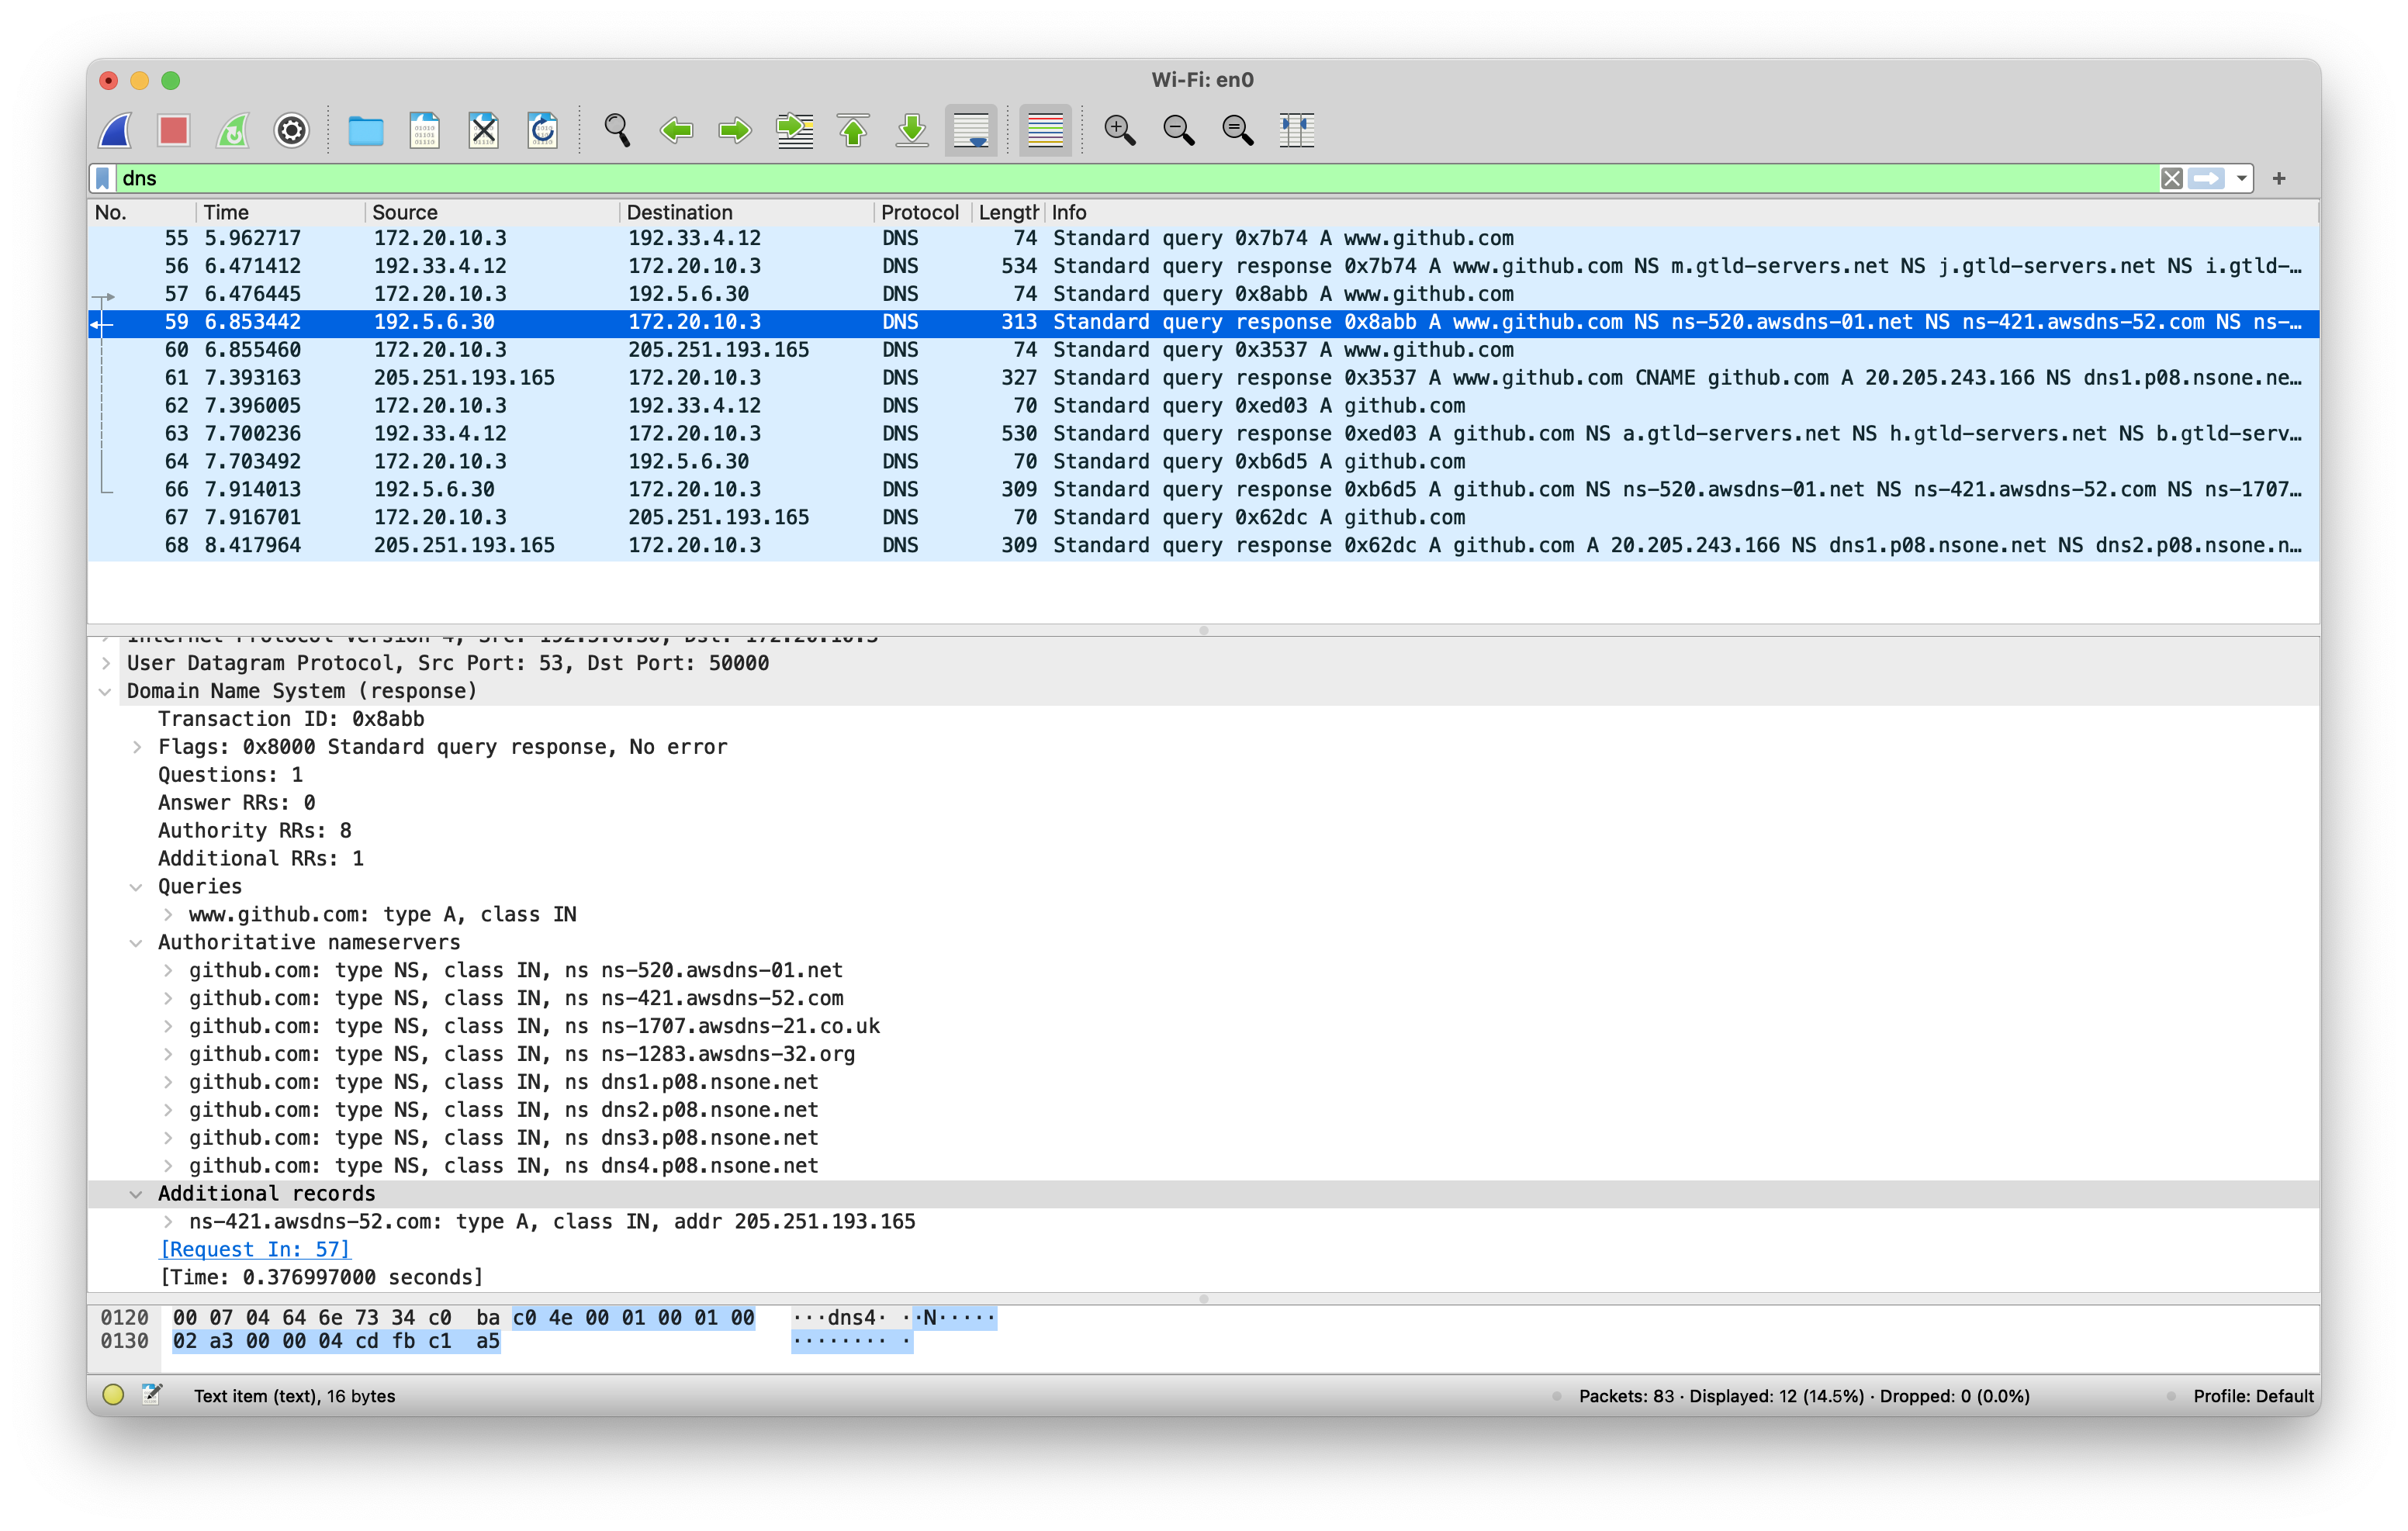
\includegraphics[height=6.2cm]{fig/w2}}
\par Now we come to ns-421.awsdns-52.com, this time, it gives us a CNAME record and an A record. Getting the IP address we want, we can happily ends the query and return an answer.\\~\\
\centerline{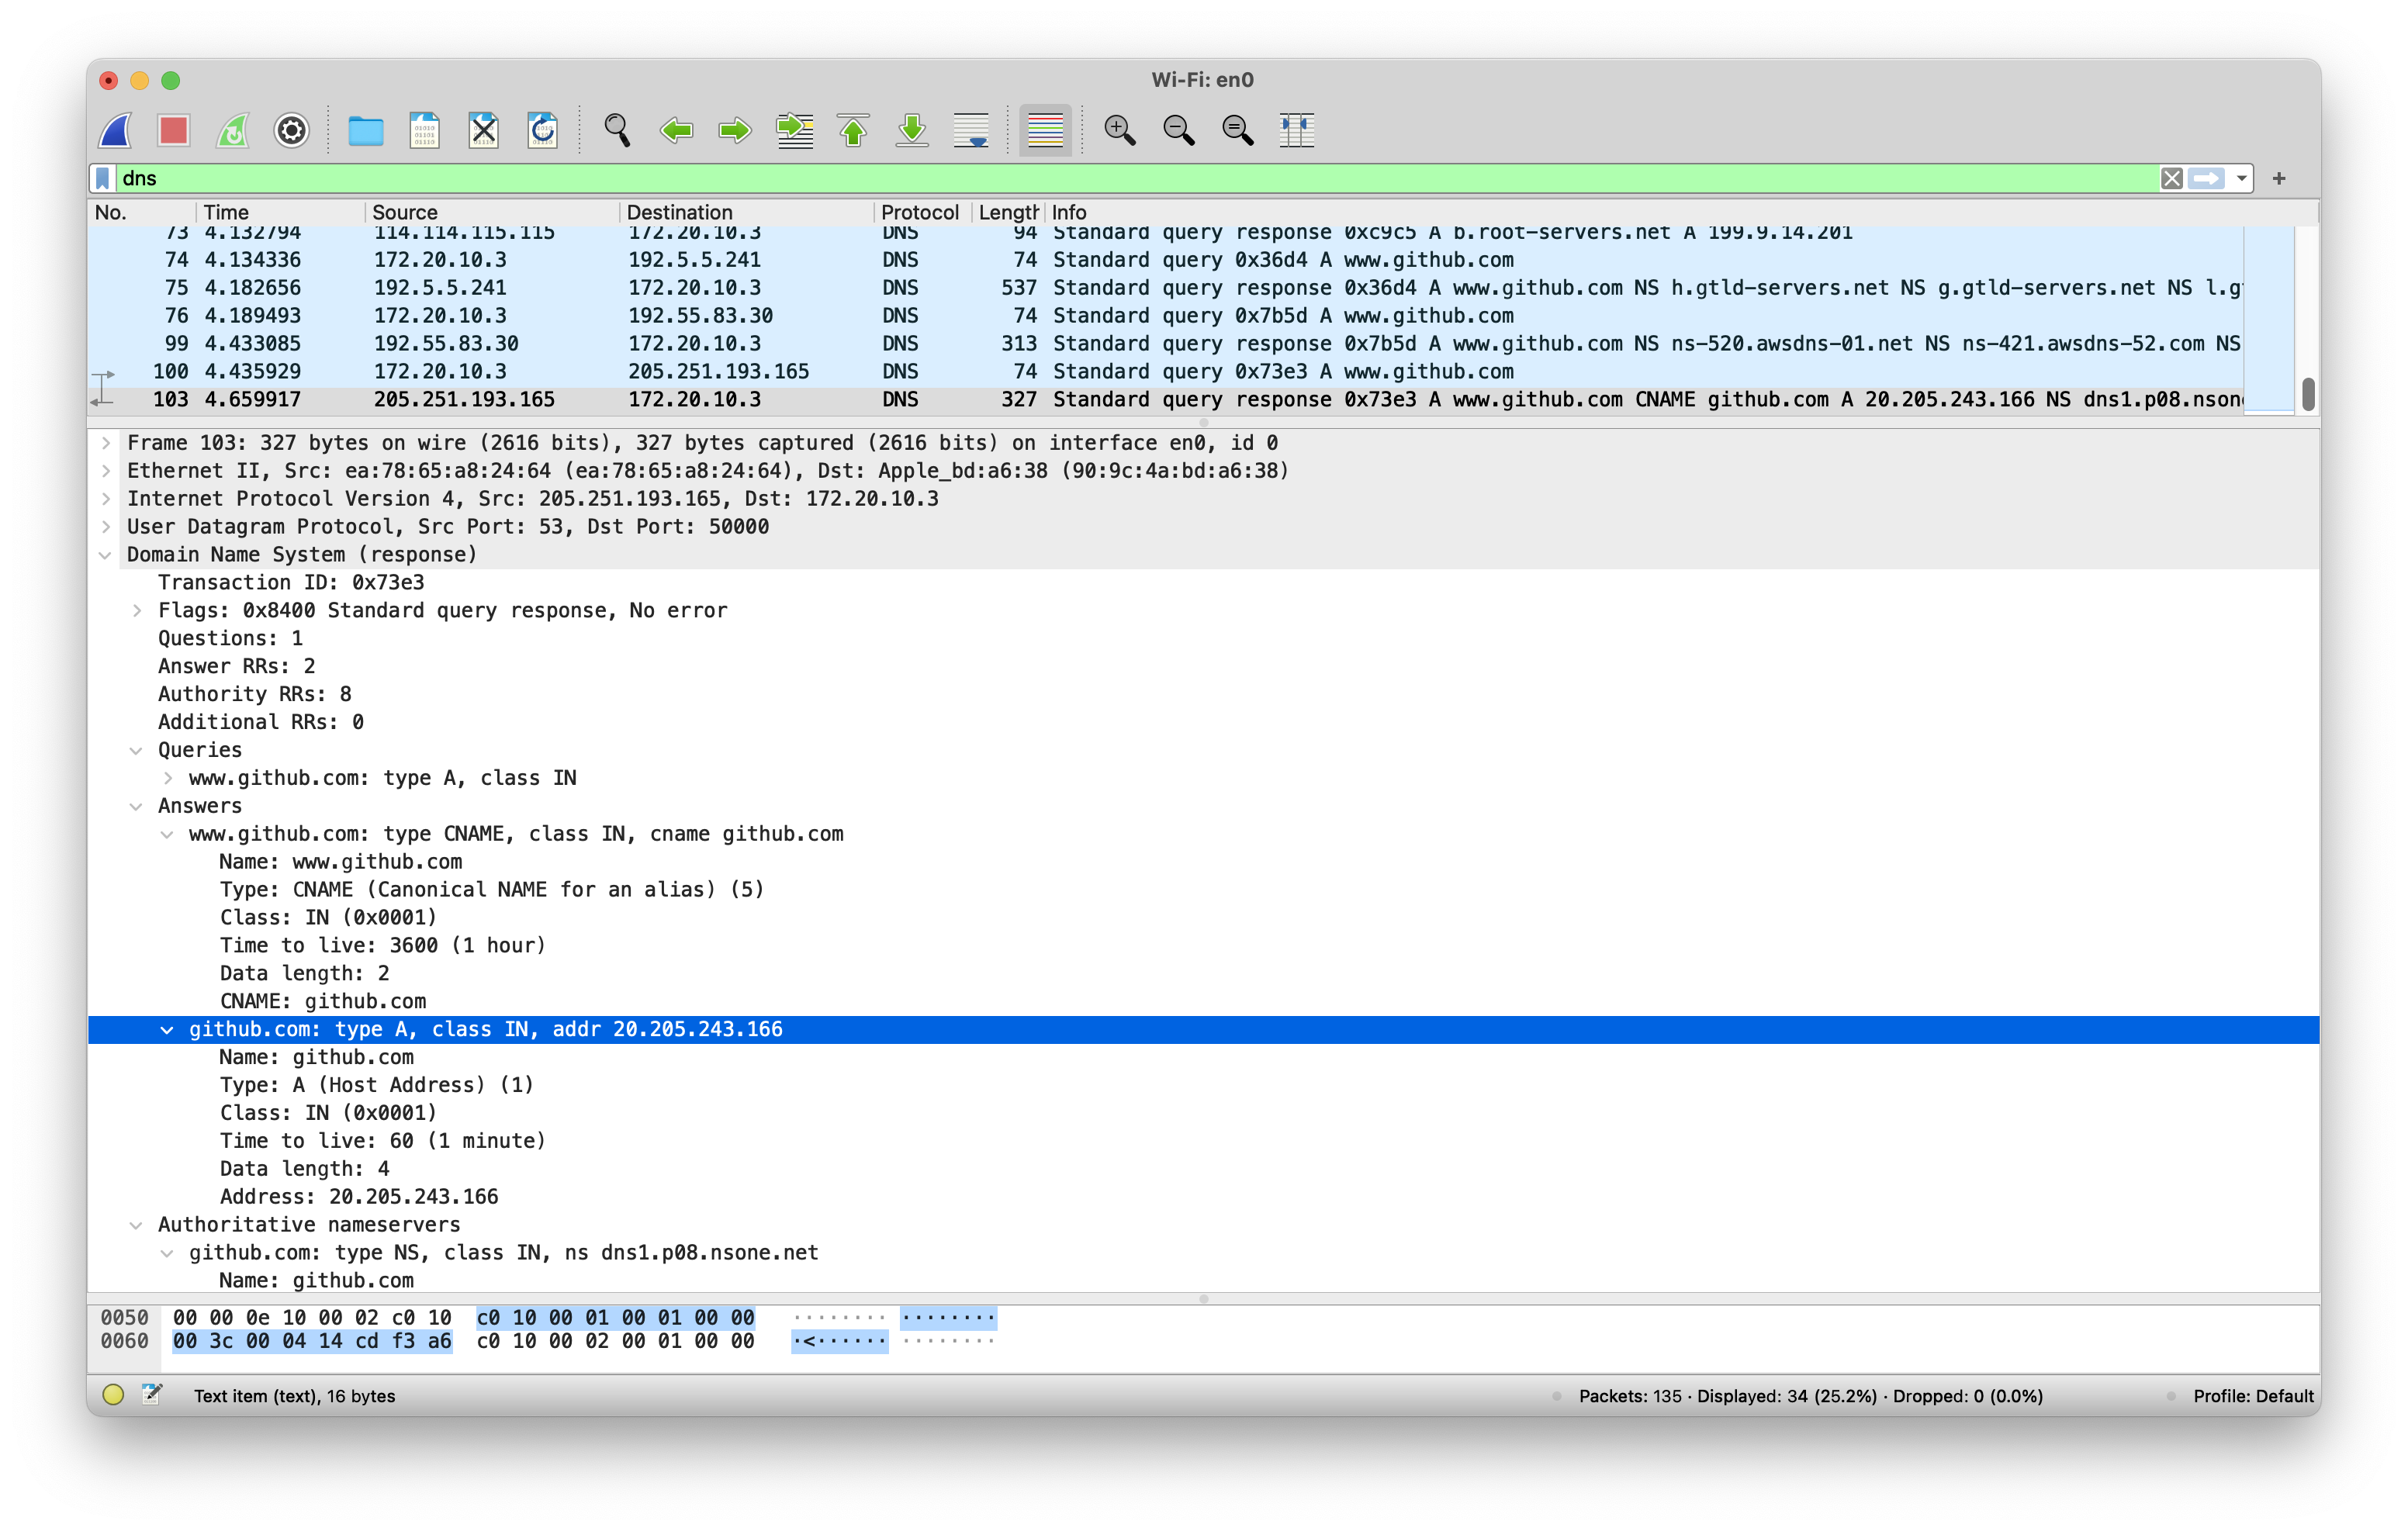
\includegraphics[height=6.2cm]{fig/w3}}


\section{Implementation Detail}

\subsection{Maintain a Cache}
\subsubsection{Human-readable}
I directly store a list of RRset related to the query name, and provide the magic function \emph{\_\_str\_\_(self)} to make it more readable. In the code I submitted, I commented lines that print the cache manager, but here's a demonstration.\\~\\
\centerline{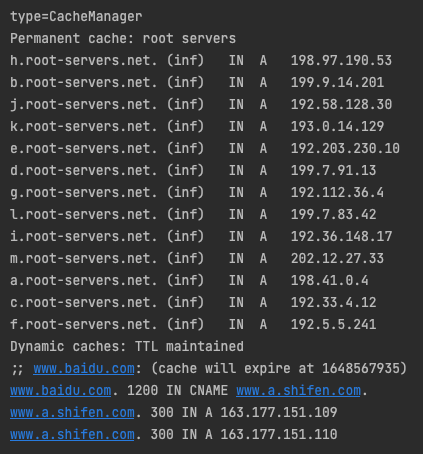
\includegraphics[width=0.4\textwidth]{fig/p111}}

\subsubsection{Record New Queries}
\begin{minted}{python}
if query_cache := self.cache_manager.read_cache(domain_name):
    logger.info('read from cache')
    return ReplyGenerator.reply(income_record, query_cache)
else:
    if resp := self.query(domain_name, self.source_ip, self.source_port):
        self.cache_manager.write_cache(domain_name, resp)
        return ReplyGenerator.reply(income_record, resp)
    else:
        return ReplyGenerator.reply_not_found(income_record)
\end{minted}

Please check line 6, in such case, there's no previous cache, s.t. the program runs into the \emph{else} block and query the domain (iteratively, from the root servers). If the query fails (wrong domain, or timeout too many times), a reply indicates the error will be returned, otherwise, it save the list of RRset into cache and return a DNSRecord with RRset items inserted into the answer section.

\subsubsection{Manage Expired Caches}
To provide a better service, and to avoid the cache dict being too heavy, we tend to delete the expired cache items dynamically, say, since TTL is in the unit of second, we run a check once a second, which checks the timestamps indicating the min TTL in a group of RRsets and delete the expired ones. Since the cache is not that large indeed, this $\mathcal{O}(n)$ check is fair enough.
\begin{minted}{python}
def __init__(self):
    ...
    # stand-alone thread for checking and deleting the cache that passes TTL
    _thread.start_new_thread(self.daemon_ttl, ())

def daemon_ttl(self):
    while True:
        timestamp = round(datetime.now().timestamp())
        for domain in list(self.cache.keys()):
            if timestamp > self.cache[domain][1]:  # cache[domain][1] is the timestamp when the min TTL passes
                del self.cache[domain]
        time.sleep(1)  # ttl manager updates pre second
\end{minted}
Plus, as we all know, thanks to GIL, this build-in dict is thread-safe, which means the daemon thread shall not mess up our cache. But to be more safe, I check the TTL timestamp again in \emph{read\_cache}.

\subsubsection{Reply a Cache}
\label{reply a cache}
As the screenshot shows, the first query cost 4062ms, but the second query is so fast that dig reports it cost 0ms. Also, the console printed a log \emph{read from cache}.\\~\\
\centerline{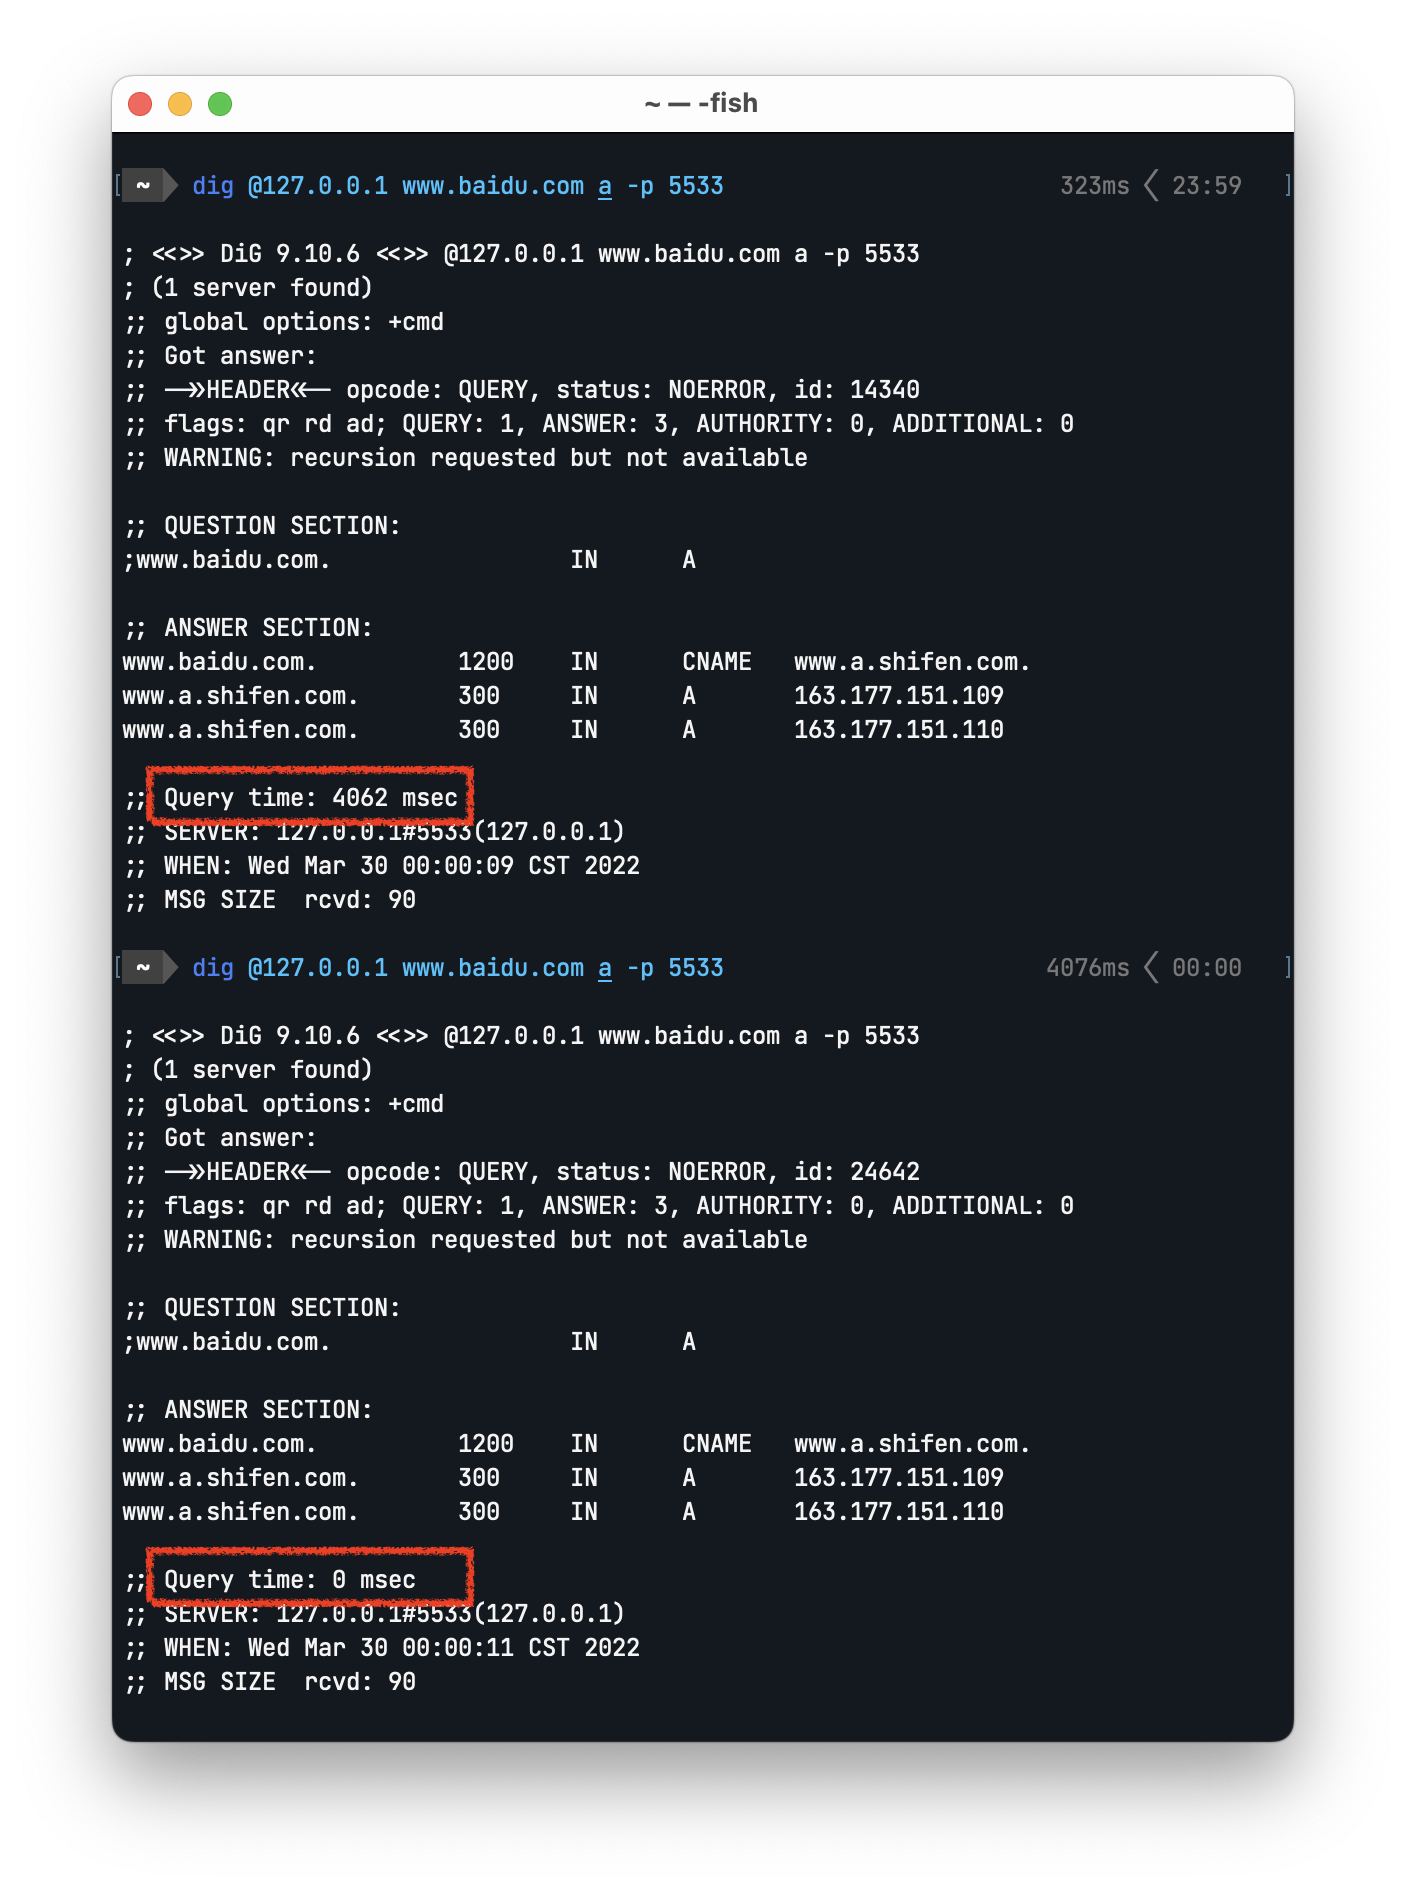
\includegraphics[width=0.5\textwidth]{fig/p112}}\\
\centerline{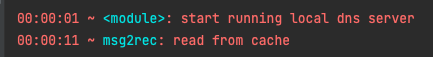
\includegraphics[width=0.4\textwidth]{fig/p113}}

\subsection{Multithreading}
The socket itself, is indeed blocking, what we need to do it the let the query itself be async, and ensure that socket messages' sending will not crash if in such OS that socket is not thread safe.
\par The first question is easy to solve. Since the class DNSHandler is iterated from threading.Thread, we can do such modifications in DNSServer\#start:
\begin{minted}{python}
def start(self):
    try:
        while True:
            message, address = self.receive()
            if message == self.last_query:
                continue
            self.last_query = message

            thread = threading.Thread(target=self.dns_handler.handle,
                                      args=(message, address, self.socket, self.lock))
            thread.daemon = True
            thread.start()
    except KeyboardInterrupt:
        logger.info('bye')
        exit(0)
\end{minted}

\par Here's a trick that records bytes \emph{last\_query}, since the dig client will send several exactly same packages if it doesn't receive the response after some time, but there's already a thread working on the query. Thus we just skip the query. But if dig sends another query that have the same query name, it is still okay, since the id in the message is different.

\par As for the socket's thread safe, a simple thread lock can be applied:
\begin{minted}{python}
@staticmethod
def reply(address, response: DNSRecord, sock: socket, lock: threading.Lock):
    with lock:
        sock.sendto(response.pack(), address)
\end{minted}


\end{document}
